\section{Discussion} \label{sec:Discussion}
\subsection{Implications}
\textbf{Cold vs hot streams:}
The assumption that the \ac{DF} of accreted particles is a $\delta$-function in action space requires them to be on a regular orbit - an assumption that is not fully (e.g. \citealp{Erkal...Pal5pert...2017}) but more closely (e.g. \citealp{Price-Whelan...chaos...2016}) satisfied for long, cold stellar streams. Already in the introduction we have mentioned, that \ac{DG} mergers usually create hot stellar streams so our particle streams in Auriga are dynamically hot and have a different, more complex \ac{DF}. Our results show that trying to constrain the gravitational potential by assuming accreted \acp{GC} from one progenitor should cluster in action space does not work. Observers who want to constrain the potential of external galaxies by action-based modelling of tracers need to take this into account and develop this more complex \acp{DF}.

\\\textbf{Integrals of motion:} We find that the integrals of motion, i.e. actions and energy, are not constant during the merger and in their time individual evolution even though the total time evolution stays rather constant. This is also due to more complex perturbations in the accretion process but there could also be dark substructure in the halo which disturbs the orbits.


\subsection{Actions of observed dwarf galaxy remnants}
It is import to compare results from analysis simulations to observations. One test is looking at our Galaxy, where we have 6D phase space information available, e.g. with \textit{Gaia} \citep{Gaia...mission...2016, GaiaDR2...overview...2018}, and to see how remnants of a \ac{DG} merger are distributed in action space.

Recently, Gaia-Enceladus \citep{Enceladus....Helmi...2018}, also found by \citet{Belokurov....Sausage...2018, Myeong...SausageGCs...2018} as \textit{Gaia Sausage}, was discovered in the \textit{Gaia} data as an overdensity in the Toomre diagram. These are remnant stars of a merger approximately \SI{10}{Gyr} ago (comparable to prog4) with a mass ratio of 0.24. In contrary to the Sagittarius \ac{DG} we have precise 6D information from \textit{Gaia} DR2 about Gaia-Enceladus which we need to calculate the actions. 

\citet{Enceladus....Helmi...2018} found Gaia-Enceladus stars in the solar neighbourhood ($d < \SI{2.5}{kpc}$) by selecting them in energy-angular momentum space with $ −1500 < L_z < \SI{150}{kpc.km.s^{-1}}$ and $E >−1.8\cdot 10^5\SI{}{km^2.s^{-2}}$ assuming a logarithmic halo, a \ac{MN} disk and a Hernquist bulge for the \ac{MW} potential.

\iffalse ich weis waere gut aber jetzt nicht mehr
\textbf{Excursion: coordinate transformations}
private communication with Wilma Trick
\fi
\begin{figure}[htbp]
\captionsetup{format=plain}
    \centering
    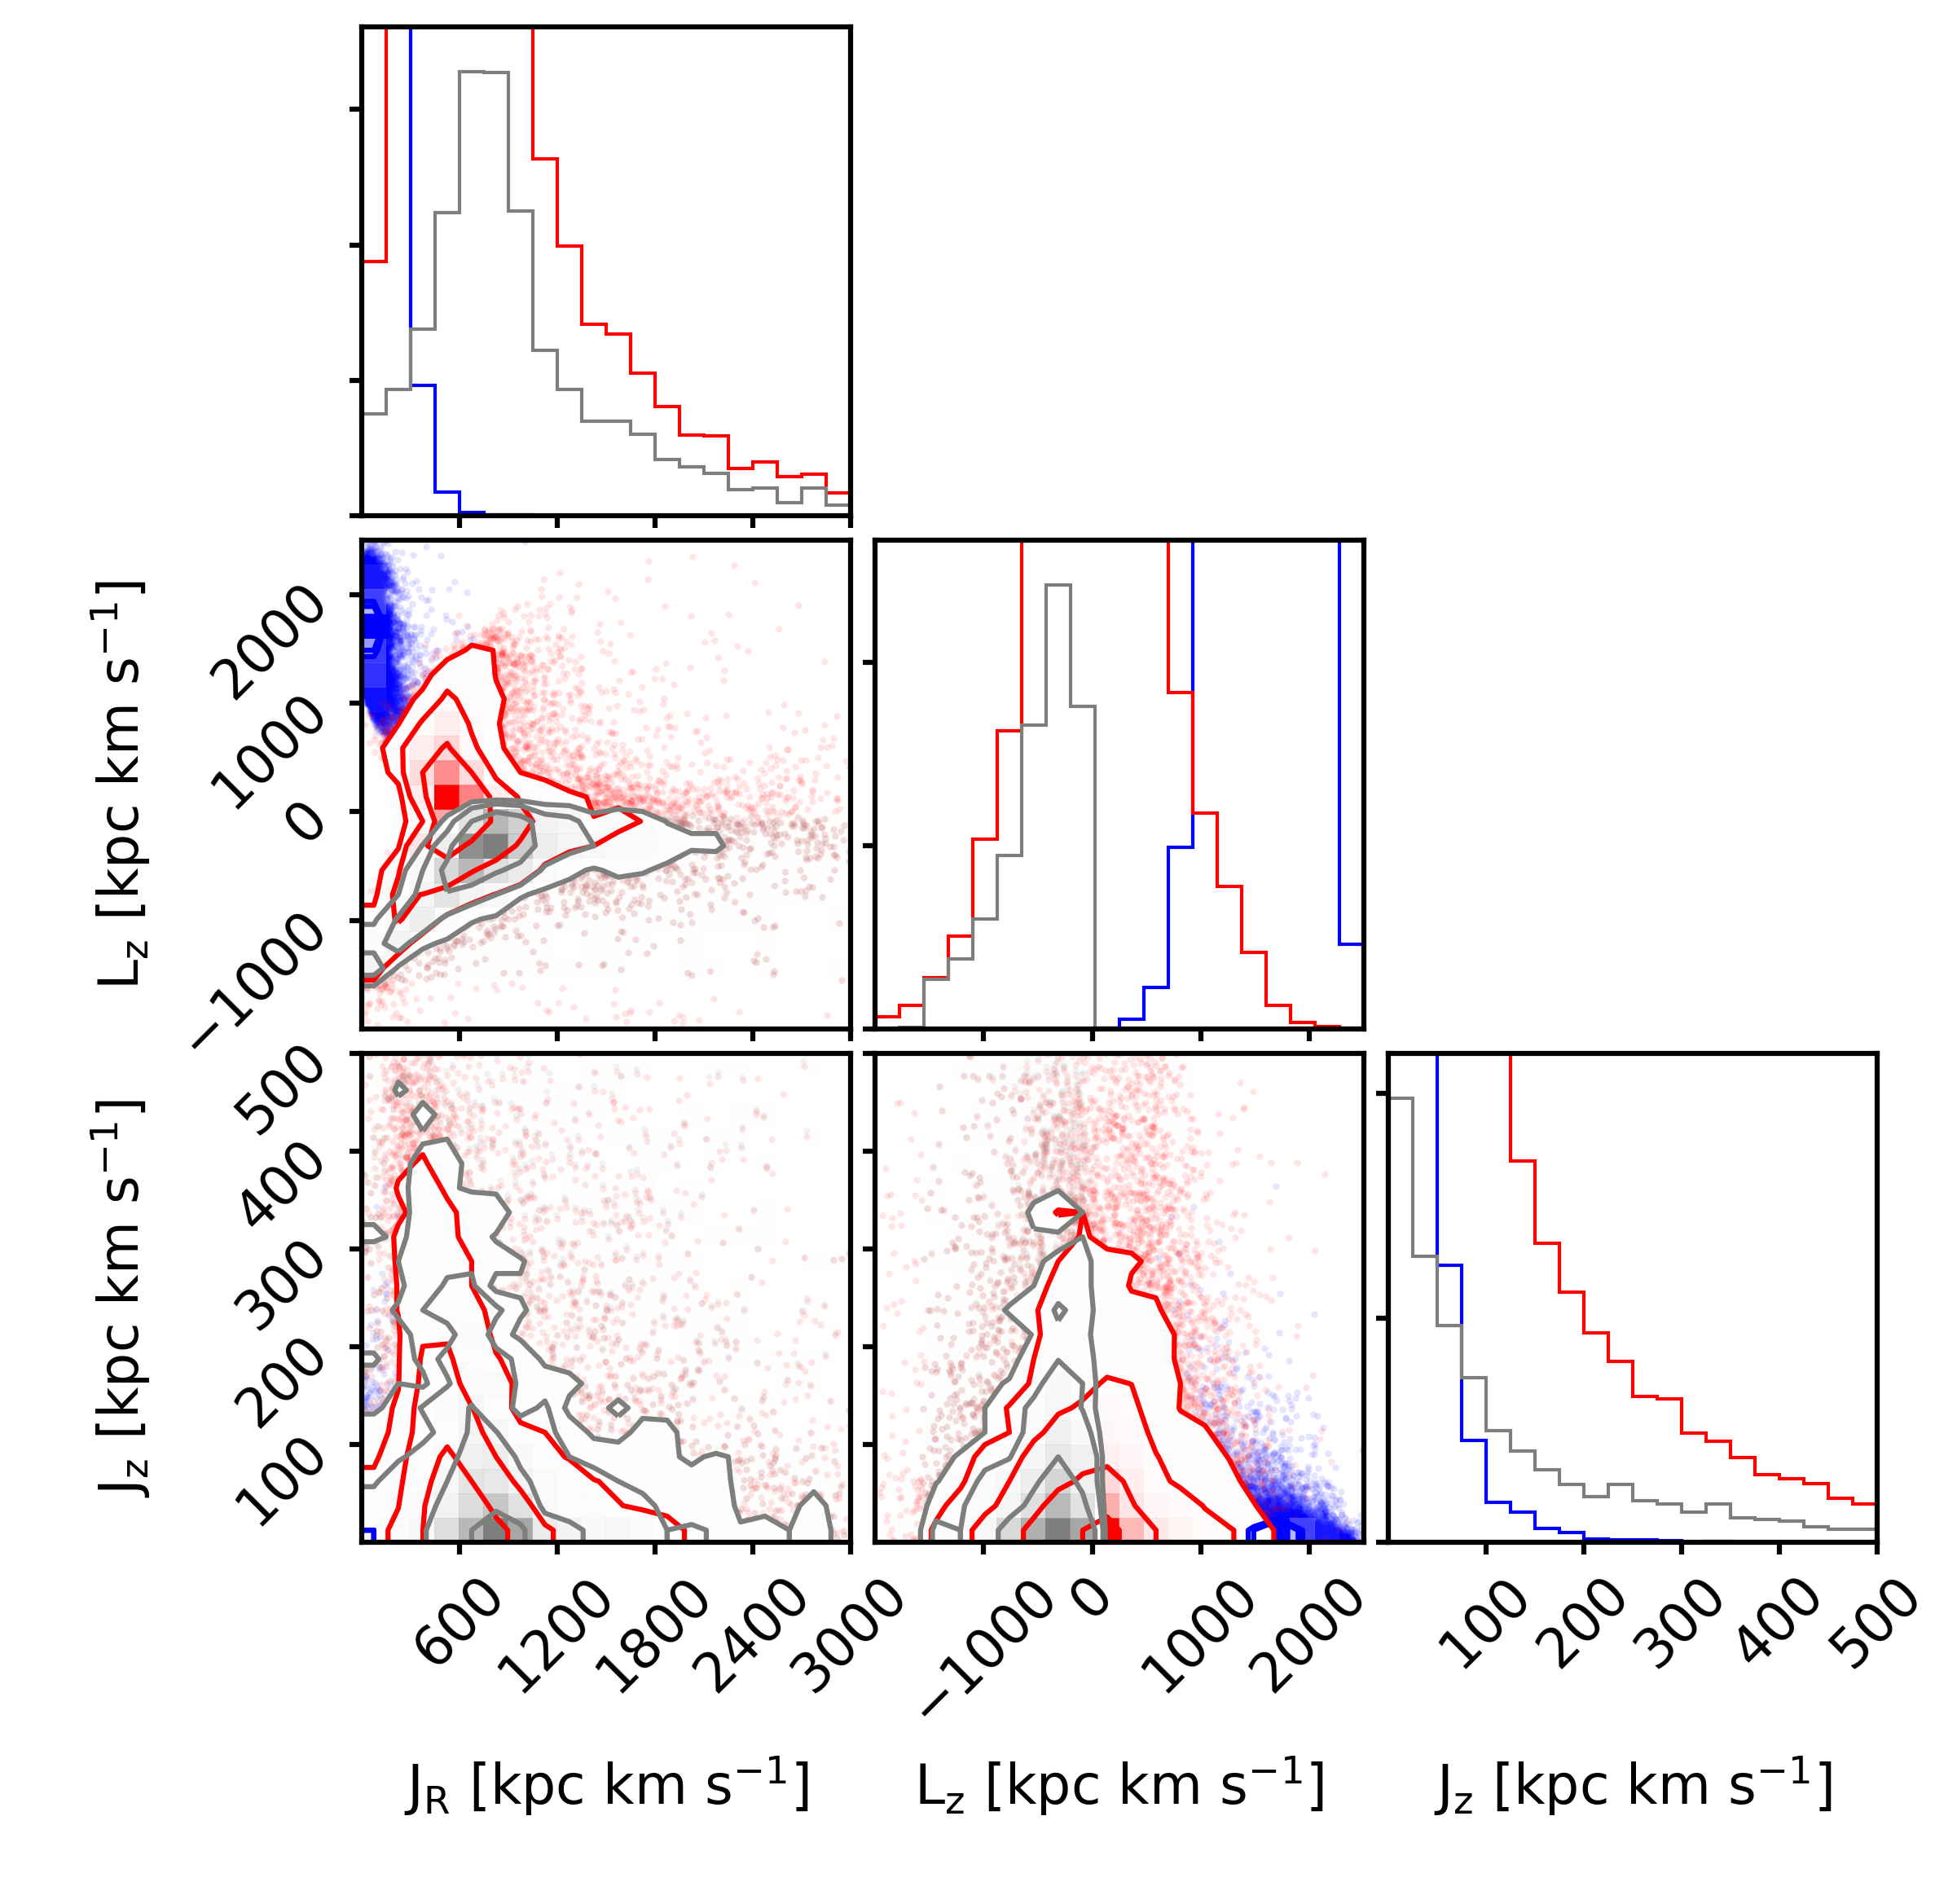
\includegraphics[width=1.0\textwidth]{plots/Discussion/Gaia_all_actions.png}
    \caption{\textit{Gaia}-Enceladus stars in action space in the \texttt{MWPotential2014} \citep{Bovy...galpy...2015}. The data is taken from \textit{Gaia} DR2 \citep{GaiaDR2...overview...2018} in the \ac{MW} within $d = 1/\omega <\SI{2.5}{kpc}$. In blue, actions of disk stars are plotted. The halo including some of the thick disk stars is red. \textit{Gaia}-Enceladus stars are plotted in grey. Disk and halo are clearly distinguishable in angular momentum and also in radial action. \textit{Gaia}-Enceladus is not distinguishable from the halo as it makes up a significant part of it. It has a negative $L_z$ therefore it is counterrotating. It is also very spread out in action space so we cannot detect any sharp features.}
    \label{fig:Gaia_Enceladus_actions}
\end{figure}
In Figure \ref{fig:Gaia_Enceladus_actions}, we show actions of the disk, halo and \textit{Gaia}-Enceladus calculated in the \texttt{MWPotential2014} \citep{Bovy...galpy...2015}. We calculate its actions also in other potentials such as the \ac{MW} potential from \citet{McMillan...MWpot...2017} and the same potential \citet{Enceladus....Helmi...2018} applied for their analysis. The distribution does not change. The remnants are neither distinguishable from the halo nor do they make a sharp feature in any of the actions. This tells us that even if there was more dynamical information contained in these stars shortly after the merger, this information vanishes over time. This confirms our findings that actions of objects accreted from a \ac{DG} merger cannot be seen as sharp features after some evolution. 

\subsection{Context in recent research and literature}
\textbf{\acp{GC} formation in cosmological simulations} \\Timo Halbesma (PhD student at the MPA) is working on extracting \acp{GC} in the Auriga simulations which have proper physical properties and physically motivated formation recipes. An improvement to this work would e.g. be that he looks for \acp{GC} which consist of more than one particle and evolve together as the mass of one stellar particle lies at the very low end of the \ac{GC} mass regime. Properly selected \acp{GC} could clump in action space because their orbits might stay (physically motivated) constant and therefore they could be used to tune the potential right. \\
The E-MOSAICS simulation suite \citep{Pfeffer...E-MOSAICS...2018, Kruijssen...E-MOSAICS.MW..2018} are zoom-in simulations of the cosmological EAGLE \citep{Schaye...EAGLE...2015} simulations which have implemented models describing the formation, evolution, and disruption of star clusters. In these simulations, Meghan Hughes (PhD student at ESO/LJMU) works on modelling the potential and Sebastian Trujillo-Gomez (Postdoc at ARI) investigates the kinematics of the \acp{GC}. 
\\\\
\textbf{Constraining gravitational potential}\\
There are attempts of applying adaptive dynamics or dynamical modelling with \acp{GC} to the \ac{MW}.
\begin{itemize}
\item \textbf{\acp{DF} of \acp{GC}} \citet{Posti...MWmassGCs...2019} model the \ac{MW}'s \ac{GC} system with two \acp{DF}, to match the two populations in the disk and the halo. This model constraints the phase-space distribution, the Galactic mass and the shape of the \ac{DM} halo. Their constraints on the \ac{MW} mass (see Table \ref{tab:MW_mass_estimations}) lies within the range of the other results. Our method differs in distinguishing \acp{GC} from different progenitors and not only into halo or disk. They use more elaborate \acp{DF} while our assumption is that the \ac{DF} is a $\delta$-function.
\item \textbf{Sharpen stellar streams in simulations to find true potential} \citet{Sanderson...streams..adaptivedyn...2015, Sanderson...gravpotstreams...2017} investigate stellar streams in cosmological simulations (Aquarius) in action space and try to constrain the gravitational potential by maximizing the amount of clustering. They are successful and can recover the mass profiles. This is very similar to this work. However, they use narrow stellar streams, which are on cold orbits, as tracers while we use \acp{GC} accreted from a dynamically hotter progenitor. This could be the reason that their method gives positive results while ours does not constrain the potential.
\item \textbf{N-body simulations of accretion of satellites} \citet{Jean-Baptiste...accactionspace...2017} carried out N-body simulations on merger with satellites including kinematical heating, tidal effects and dynamical friction. In $E-L_z$ space, they found substructure, as expected, but also found multiple satellites to overlap - like prog3 and prog4 in our analysis in action space. Furthermore they found that energy and angular momentum are not conserved during a merger - another conclusion we find in our work in energy and action space. Their work sides with our results. 
\end{itemize}

\subsection{Caveats}
There are a few assumptions and problems in the course of the investigations which might have influenced the results.
\\\\\textbf{GC selection}
One of the main problems in the analysis is the \ac{GC} selection. Auriga does not resolve \acp{GC} and therefore we need to make assumptions and select \ac{GC} candidates. We applied a very simple recipe which only excluded simulated particles as \ac{GC} candidates which were in a snapshot in a regime where the stellar disk was very dense and could have destroyed the \ac{GC}. We carried out the same analysis for different subsets (selected both randomly and specifically through some cuts in the distribution or kinematics). The results were comparable to the ones presented, i.e. the standard deviation in different potentials (Figure \ref{fig:a_NFW_diagnostic_plots}) and the action evolution for all three progenitors (Figures \ref{fig:actions_time_evolution_prog2} - \ref{fig:actions_time_evolution_prog4}) showed the same results. However, it would be interesting to see if the properly selected \acp{GC} (see Section above) follow the same trends.
\\\\\textbf{Potential fit}
As we have discussed in Section \ref{subsec:wrong_pot_fit}, there are a few problems with the potential fit. The bulge-disk decomposition probably underestimates the disk and creates a flaring spatial selection effect. For each component, the model differs from the data especially in the center. This is due to the choice of binning the data, fitting routines, the assumption of spherical or axisymmetry, the simplified potential model consisting of only three analytic building blocks etc. In total, the potential is good enough for the course of our investigations but, as one of the next steps, should be improved.

\subsection{Future Work}
There are a lot of things which we could not investigate or we had to make compromises on due to the time limitations of this thesis. Big issues which we already discussed are with the potential model and, to a smaller extent, with the \ac{GC} selection. Improving these recipes would make our analysis more robust. The potential fit could be enhanced by not only fitting spatial properties but also kinematic ones, e.g. the circular velocity. As the vertical profile seems not so well reproduced by the assumed model family, it might be worth experimenting with other disk profiles, superpositions of several \ac{MN} disks, or non-spherical halo shapes.

\\\\
\texttt{galpy} and \texttt{AGAMA} \citep{Vasiliev...AGAMA...2019} can in principle calculate actions for \textit{N}-body simulations directly without the need of an analytic gravitational potential. We should compare if the action distribution and evolution behaves as we measured because of their nature and their physical evolution in the simulation (so the calculation of actions in a St\"aeckel Fudge or similar approach without the need of an analytic potential first and calculating them in our potential model would give similar results) or because an analytic axisymmetric potential (in general or only our fit) cannot well describe the real potential and messes these things up. Up to now, it was not possible for us to do this step due to technical issues. 

\\\\The final goal would be to find the right \ac{DF} of accreted particles which is not yet possible due to numerical (and observational) limitations. If we knew the \ac{DF}, adaptive dynamics in external galaxies should be a useful method to constrain their gravitational potential. With this true \ac{DF} and the right gravitational potential, we would know everything about the dynamics of the galaxy.

